\setchapterpreamble[u]{\margintoc}
\chapter{Ricerca degli zeri}
\labch{zeri}
%NOTE: il risultato con Newton-Raphson puo' non convergere se la derivata e' nulla (punto stazionario o punto di flesso)

%NOTE: e' meglio combinare il metodo di bisezione con il metodo di Newton-Raphson: si fa qualche ciclo di bisezione e poi si utilizza il metodo di Newton

% |c-c_n| <= 2^{-n} |b-a|, |c-c_n+1| <= |c-c_n|
% scala logaritmica -> retta, algoritmi migliori

\section{Esercizi}

%TODO:

\subsection{Esercizio 9}

\begin{marginfigure}
	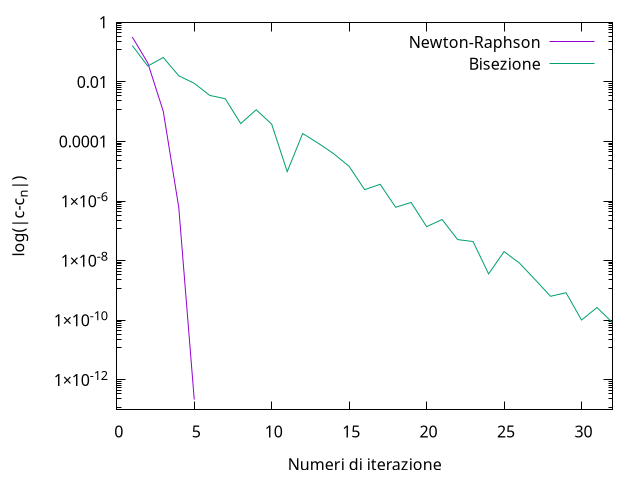
\includegraphics[width=1.5\textwidth]{roots_9_convergence_analysis.png}
	\caption{Convergenza dei due meetodi}
	\label{fig:roots_ex_9}
\end{marginfigure}

\begin{enumerate}
	\item Dato $-x^2 + x + \frac{1}{2} = 0$ le radici sono $x_{\pm}=\frac{-1 \pm \sqrt{1-4(-1)(1/2)}}{-2}=\frac{1\pm\sqrt{3}}{2}$. Dal metodo di bisezione otteniamo \texttt{1.36603} nell'intervallo $[0.8,1.6]$ come verificato dalla teoria, il medesimo risultato si ottiene per il metodo di Newton-Raphson.
	\item TODO:
    \item[3, 4] Dalla \reffig{roots_ex_9} si osserva che il metodo di bisezione converge piu' lentamente rispetto a quello di Newton-Raphson. Inoltre si osserva che il metodo di Bisezione converge linearmente ($\sim 2^{-n}$).
\end{enumerate}


\subsection{Esercizio 10}

\paragraph{Convergenza lenta} Lo zero della funzione $x^2$ e' banalmente $0$ se
consideriamo l'espressione analitica dell'errore del metodo di Newton-Raphson otteniamo: 
\[
    |0-x_{n+1}| = x_n - \frac{x_n^2}{2 x_n} = x_n - \frac{1}{2} x_n = \frac{1}{2}x_n
\]
Quindi l'errore del metodo di Newton-Raphson e' lineare in questo caso specifico.
In effetti come si puo' osservare dal file \texttt{ex\_10\_1.dat} si ottiene un valore costante di \texttt{0.5} come da teoria (a meno di errori di precisione successivi).

In conclusione la convergenza del metodo di Newton-Raphson, nonostante in generale sia quadratica, puo' essere diversa da quella prevista, a causa delle proprieta' analitiche della funzione in esame.

\paragraph{Cicli} 

Nei casi in cui si vuole studiare la convergenza del metodo di Newton-Raphson si
puo' studiare il frattale associato. Con un semplice programma python (\texttt{newton\_fractal.py}) si possono studiare le aree di convergenza del metodo data la
funzione.

TODO

\paragraph{Condizioni iniziali} Anche in questo caso studiamo i risultati e il
frattale associato alla funzione ottenendo \reffig{ex_10_3} e \reffig{newton_fractal_2}.

Dei valori iniziali relativamente simili cadono in delle regioni di convergenza 
diverse, basterebbe un leggero spostamento della condizione iniziale per ottenere uno zero differente.

Il carattere oscillatorio e' spiegabile analogamente al punto precedente.
\begin{marginfigure}
    \hspace{-2.1cm}
	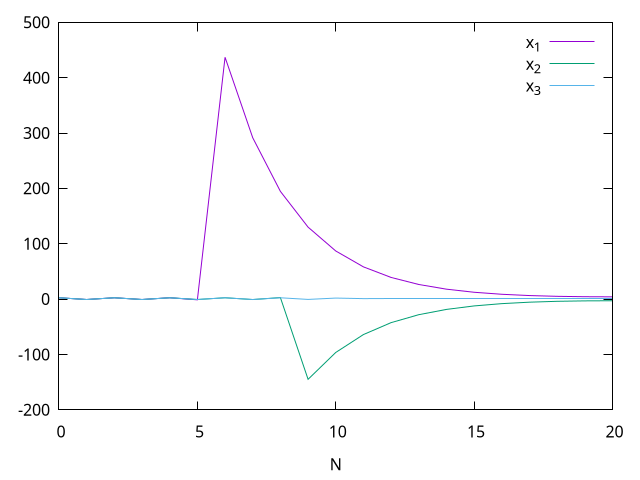
\includegraphics[width=1.5\textwidth]{initial_value_roots.png}
	\caption{Carattere oscillatorio del metodo di Newton per le condizioni iniziali del terzo punto, $x_1, x_2, x_3$ sono i valori in ordine proposti nelle note}
	\label{fig:ex_10_3}
\end{marginfigure}

\begin{marginfigure}
    \hspace{-2.1cm}
	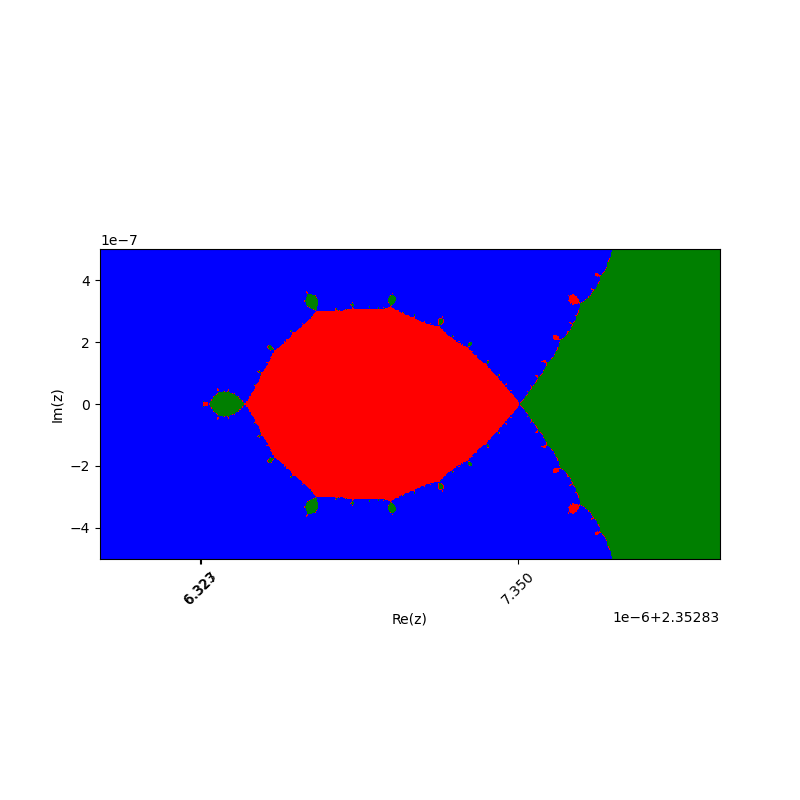
\includegraphics[width=1.5\textwidth]{newton_fractal.png}
	\caption{Frattale di Newton associato al terzo punto, colori diversi corrispondono a zeri diversi, si noti che due dei valori sono quasi sovrapposte in questa scala}
	\label{fig:newton_fractal_2}
\end{marginfigure}

\subsection{Esercizio 11}

\paragraph{Implementazione}

L'implmentazione e' diretta: 
\begin{lstlisting}[language=C++]
  // ... Asserts e definizione della funzione

  int n_coeffs = coefficients.Rows() - 1;

  auto coeffs_matrix = tensor::Tensor<T>::SMatrix(n_coeffs);

  // Si riempie la matrice 
  for (int i = 0; i < n_coeffs; i++) {
    if (i < n_coeffs - 1) {
      coeffs_matrix(i, i + 1) = 1.0;
    }

    coeffs_matrix(n_coeffs - 1, i) = -coefficients(i) / coefficients(n_coeffs);
  }

  // Si utilizza il Deflation Method con un termine correttivo alpha
  auto solution = eigen::PowerMethodDeflation(coeffs_matrix, n, alpha);

  // Sorting e return...
\end{lstlisting}

\paragraph{Analisi risultati}

Dopo aver aggiunto uno shift del \textit{Power method} rispettivamente di $\alpha_1=0.01, \alpha_2=0.1$. Si ottengono i seguenti valori

\begin{lstlisting}

\end{lstlisting}

\begin{minipage}{0.45\textwidth}
\lstset{basicstyle=\ttfamily\small, frame=single}
\begin{lstlisting}
Zeri di Legendre:
-0.973907
-0.865063
-0.67941
-0.433395
-0.148874
0.148874
0.433395
0.67941
0.865063
0.973907
Check:
2.59017e-07
4.42142e-08
-1.97815e-11
-5.12745e-11
7.348e-09
1.31299e-09
8.9706e-12
2.01226e-11
-4.42287e-08
-2.59039e-07
\end{lstlisting}
\end{minipage}
\hfill
\begin{minipage}{0.45\textwidth}
\lstset{basicstyle=\ttfamily\small, frame=single}
\begin{lstlisting}
Zeri di Hermite: 
-2.3506
-1.33585
0.00120427
0.436077
1.33585
2.3506
0.433395
-0.433395
0
7.16395e-322
Check:
1.81899e-12
-6.25278e-13
-119.999
-3.86358e-13
1.02318e-12
1.81899e-12
\end{lstlisting}
\end{minipage}

L'algoritmo funziona dunque correttamente.

